%%%%%%%%%%%%%%%%%%%%%%%%%%%%%%%%%%%%
% Slide options
%%%%%%%%%%%%%%%%%%%%%%%%%%%%%%%%%%%%

% Option 1: Slides with solutions

\documentclass[slidestop,compress,mathserif]{beamer}
\usepackage{booktabs}
\usepackage{array}
\newcommand{\soln}[1]{\textit{#1}}
\newcommand{\solnGr}[1]{#1}

% Option 2: Handouts without solutions

%\documentclass[11pt,containsverbatim,handout]{beamer}
%\usepackage{booktabs}
%\usepackage{array}
%\usepackage{pgfpages}
%\pgfpagesuselayout{4 on 1}[letterpaper,landscape,border shrink=5mm]
%\newcommand{\soln}[1]{ }
%\newcommand{\solnGr}{ }

%%%%%%%%%%%%%%%%%%%%%%%%%%%%%%%%%%%%
% Style
%%%%%%%%%%%%%%%%%%%%%%%%%%%%%%%%%%%%
%%%%%%%%%%%%%%%%%%%%%%%%%%%%%%%%%%%%%%%%%%%%%%%%%%%%%%%%%%%%%%%%%%%%%%%%
% MA213/214 shared slide style
%
% "Calm & Cool" palette + content-type callout boxes.
% Overhauled (2026) from the original OpenIntro/metropolis style:
%   - all OpenIntro visual branding removed (logo, grid, colors)
%   - a low-key cool palette (see colors below)
%   - tcolorbox callout boxes so students recognize content types
% See common/README.md for the command cheat-sheet.
%%%%%%%%%%%%%%%%%%%%%%%%%%%%%%%%%%%%%%%%%%%%%%%%%%%%%%%%%%%%%%%%%%%%%%%%

\usetheme{metropolis}

%%%%%%%%%%%%%%%%
% Packages
%%%%%%%%%%%%%%%%

\usepackage{geometry}
\usepackage{graphicx}
\usepackage{amssymb}
\usepackage{epstopdf}
\usepackage{amsmath}  	% this permits text in eqnarray among other benefits
\usepackage{url}		% produces hyperlinks
\usepackage{hyperref}	% allows for color usage in tables
\usepackage[english]{babel}
\usepackage[latin1]{inputenc}
\usepackage{colortbl}	% allows for color usage in tables
\usepackage{multirow}	% allows for rows that span multiple rows in tables
\usepackage{color}		% this package has a variety of color options
\usepackage{pgf}
\usepackage{calc}
\usepackage{ulem}
\usepackage{multicol}
\usepackage{textcomp}
\usepackage{txfonts}
\usepackage{listings}
\usepackage{tikz}
\usepackage{array}
\usepackage{wasysym}
\usepackage{fancyvrb}
\usepackage{etoolbox}             % \ifstrempty for optional box subtitles
\usepackage[most]{tcolorbox}      % content-type callout boxes
\tcbuselibrary{listings}          % R-code block (\begin{rblock})
\usepackage{fontawesome5}         % box icons

%%%%%%%%%%%%%%%%
% Remove navigation symbols
%%%%%%%%%%%%%%%%

\setbeamertemplate{navigation symbols}{}

%%%%%%%%%%%%%%%%
% "Calm & Cool" palette
%%%%%%%%%%%%%%%%

% chrome / structure / body
\definecolor{ccSlate}{HTML}{2E3742}   % frametitle bar, structure, section pages (deep neutral slate)
\definecolor{ccInk}{HTML}{2B2B2B}     % body text
\definecolor{ccWash}{HTML}{FCF8F1}    % gentle warm title-slide background wash (complements the cool blues)

% example (blue)
\definecolor{ccBlue}{HTML}{2F6690}
\definecolor{ccBlueBg}{HTML}{EAF1F7}
% interactive activity / discussion (green)
\definecolor{ccGreen}{HTML}{4E8A6B}
\definecolor{ccGreenBg}{HTML}{E9F3EC}
% solution (purple)
\definecolor{ccPurple}{HTML}{6F5499}
\definecolor{ccPurpleBg}{HTML}{EFEAF6}
% worksheet / focused work (terracotta)
\definecolor{ccTerra}{HTML}{C2693E}
\definecolor{ccTerraBg}{HTML}{FAEDE4}
% formula / definition (neutral slate)
\definecolor{ccGray}{HTML}{5C6B7A}
\definecolor{ccGrayBg}{HTML}{EEF1F4}
% caution / common pitfall (brick red)
\definecolor{ccRed}{HTML}{B23A48}
\definecolor{ccRedBg}{HTML}{FAEAEC}
% key idea / takeaway (muted gold)
\definecolor{ccGold}{HTML}{9C7A28}
\definecolor{ccGoldBg}{HTML}{F7F1DF}
% learning goals / lesson outcomes (teal)
\definecolor{ccTeal}{HTML}{2C6E6B}
\definecolor{ccTealBg}{HTML}{E6F0EF}
% learning objectives (indigo)
\definecolor{ccIndigo}{HTML}{45507A}
\definecolor{ccIndigoBg}{HTML}{ECEEF4}
% R code / output (gray)
\definecolor{ccCode}{HTML}{5F5E5A}
\definecolor{ccCodeBg}{HTML}{F4F5F6}

% neutral grays kept from the original style
\definecolor{gray}{rgb}{0.5, 0.5, 0.5}
\definecolor{darkGray}{rgb}{0.3, 0.3, 0.3}
\definecolor{darkerGray}{rgb}{0.2, 0.2, 0.2}

% Backwards-compatible aliases: old OpenIntro color names now point at the
% new palette, so existing \textcolor{oiB}{...}, \hl{...}, etc. keep working.
\colorlet{oiB}{ccBlue}
\colorlet{oiG}{ccGreen}
\colorlet{hlblue}{ccBlue}
\colorlet{rubineRed}{ccRed}
\colorlet{irishGreen}{ccGreen}
\colorlet{lightGreen}{ccGreen}

%%%%%%%%%%%%%%%%
% Restyle metropolis with the Calm & Cool chrome
%%%%%%%%%%%%%%%%

\metroset{block=fill}

\setbeamercolor{normal text}{fg=ccInk, bg=white}
\setbeamercolor{structure}{fg=ccSlate}
\setbeamercolor{alerted text}{fg=ccBlue}
\setbeamercolor{example text}{fg=ccGreen}
\setbeamercolor{frametitle}{bg=ccSlate, fg=white}
\setbeamercolor{progress bar}{fg=ccBlue}
\setbeamercolor{title separator}{fg=ccBlue}
\setbeamercolor{title}{fg=ccSlate}
\setbeamercolor{subtitle}{fg=ccBlue}
\setbeamercolor{author}{fg=ccInk}
\setbeamercolor{institute}{fg=ccGray}
\setbeamercolor{date}{fg=ccGray}
\setbeamercolor{section title}{fg=ccSlate}
\setbeamercolor{standout}{fg=white, bg=ccSlate}

% Section pages sit on the same warm wash as the title slide. We keep
% metropolis's section-title styling and just paint a full-page ccWash
% background behind it (needs >=2 pdflatex passes for the current-page node).
\setbeamertemplate{section page}{%
  \begin{tikzpicture}[remember picture, overlay]
    \fill[ccWash] (current page.south west) rectangle (current page.north east);
  \end{tikzpicture}%
  \centering
  \begin{minipage}{22em}
    \raggedright
    \usebeamercolor[fg]{section title}%
    \usebeamerfont{section title}%
    \insertsectionhead\\[-1ex]
    \usebeamertemplate*{progress bar in section page}%
    \par
  \end{minipage}\par
  \vspace{\baselineskip}
}

%%%%%%%%%%%%%%%%
% Custom inline text commands (recolored to the palette)
%%%%%%%%%%%%%%%%

% degree
\newcommand{\degree}{\ensuremath{^\circ}}

% cite
\newcommand{\ct}[1]{
\vfill
{\tiny #1}}

\newcommand{\NamedNote}[2]{
\rule{2.5cm}{0.25pt} \\ \textit{\footnotesize{\textcolor{rubineRed}{#1:} \textcolor{darkerGray}{#2}}}}

% Note
\newcommand{\Note}[1]{
\rule{2.5cm}{0.25pt} \\ \textit{\footnotesize{\textcolor{rubineRed}{Note:} \textcolor{darkerGray}{#1}}}}

% Remember
\newcommand{\Remember}[1]{\textit{\scriptsize{\textcolor{ccTerra}{Remember:} #1}}}

% expected counts
\newcommand{\ex}[1]{\textit{\textcolor{ccBlue}{#1}}}

% red
\newcommand{\red}[1]{\textit{\textcolor{rubineRed}{#1}}}

% pink
\newcommand{\pink}[1]{\textit{\textcolor{rubineRed!90!white!50}{#1}}}

% green
\newcommand{\green}[1]{\textit{\textcolor{irishGreen}{#1}}}

% orange
\newcommand{\orange}[1]{\textit{\textcolor{ccTerra}{#1}}}

% links: webURL, webLink, appLink
\newcommand{\webURL}[1]{\urlstyle{same}{ \textit{\textcolor{darkGray}{\url{#1}}}}}
\newcommand{\webLink}[2]{\href{#1}{\textcolor{darkGray}{{#2}}}}
\newcommand{\appLink}[2]{\href{#1}{\textcolor{white}{{#2}}}}

% mail
\newcommand{\mail}[1]{\href{mailto:#1}{\textit{\textcolor{darkGray}{#1}}}}

% highlighting: hl, hlGr, mathhl
\newcommand{\hl}[1]{\textit{\textcolor{hlblue}{#1}}}
\newcommand{\hlGr}[1]{\textit{\textcolor{lightGreen}{#1}}}
\newcommand{\mathhl}[1]{\textcolor{hlblue}{\ensuremath{#1}}}

%%%%%%%%%%%%%%%%
% Structural helpers (unchanged from the original)
%%%%%%%%%%%%%%%%

% two col: two columns
\newenvironment{twocol}[4]{
\begin{columns}[c]
\column{#1\textwidth}
#3
\column{#2\textwidth}
#4
\end{columns}
}

% slot (for probability calculations)
\newenvironment{slot}[2]{
\begin{array}{c}
\underline{#1} \\
#2
\end{array}
}

% pr: left and right parentheses
\newcommand{\pr}[1]{
\left( #1 \right)
}

% cancel
\newcommand{\cancel}[1]{%
    \tikz[baseline=(tocancel.base)]{
        \node[inner sep=0pt,outer sep=0pt] (tocancel) {#1};
        \draw[red, line width=0.5mm] (tocancel.south west) -- (tocancel.north east);
    }%
}

% removepagenumbers
\newcommand{\removepagenumbers}{%
  \setbeamertemplate{footline}{}
}

% change margin
\newenvironment{changemargin}[2]{%
\begin{list}{}{%
\setlength{\topsep}{0pt}%
\setlength{\leftmargin}{#1}%
\setlength{\rightmargin}{#2}%
\setlength{\listparindent}{\parindent}%
\setlength{\itemindent}{\parindent}%
\setlength{\parsep}{\parskip}%
}%
\item}{\end{list}}

% footnote
\long\def\symbolfootnote[#1]#2{\begingroup%
\def\thefootnote{\fnsymbol{footnote}}\footnote[#1]{#2}\endgroup}

% commands from the book
\newenvironment{data}[1]{\texttt{#1}}{}
\newenvironment{var}[1]{\texttt{#1}}{}
\newenvironment{resp}[1]{\texttt{#1}}{}

%%%%%%%%%%%%%%%%
% Content-type callout boxes (tcolorbox)
%
% Each type has a colored title strip (icon + label) over a light fill.
% Color = content type; the label + icon reinforce it (so the cue does
% not rely on color alone).
%%%%%%%%%%%%%%%%

\tcbset{
  cccallout/.style 2 args={
    enhanced, breakable=false,
    colback=#2, colframe=#1, colbacktitle=#1, coltitle=white,
    fonttitle=\bfseries\footnotesize,
    boxrule=0.6pt, arc=2.5pt, outer arc=2.5pt,
    left=5pt, right=5pt, top=3pt, bottom=3pt, boxsep=2pt,
    toptitle=2pt, bottomtitle=2pt, lefttitle=5pt,
    before skip=5pt, after skip=5pt,
  },
}

% One-off / collection of examples (blue): \workedexample[subtitle]{body}.
% (Named \workedexample, not \example, because beamer defines \example.)
\newtcolorbox{examplebox}[1][]{cccallout={ccBlue}{ccBlueBg},
  title={\faIcon{lightbulb}~~Example\ifstrempty{#1}{}{ \textmd{---}\ #1}}}
\newcommand{\workedexample}[2][]{\begin{examplebox}[#1]#2\end{examplebox}}

% Running-example header (blue): \examplehead{name} at the top of each frame of a
% multi-slide running example. A one-off or a collection of examples uses the
% \workedexample box above instead.
\newcommand{\examplehead}[1]{%
  \vspace{-0.4em}\par\noindent\tcbox[on line, colback=ccBlue, colframe=ccBlue, coltext=white,
    boxrule=0pt, arc=2pt, left=5pt, right=5pt, top=1pt, bottom=1pt,
    box align=base, nobeforeafter]{\footnotesize\bfseries\faIcon{lightbulb}\,Running example}%
  \ifstrempty{#1}{}{\enspace{\footnotesize\bfseries\textcolor{ccBlue}{#1}}}%
  \par\nobreak\vspace{-0.6em}{\color{ccBlue}\rule{\linewidth}{0.7pt}}\par\nobreak\vspace{-0.8em}}

% Interactive activity (green): \activity[subtitle]{body}
\newtcolorbox{activitybox}[1][]{cccallout={ccGreen}{ccGreenBg},
  title={\faIcon{users}~~Activity\ifstrempty{#1}{}{ #1}}}
\newcommand{\activity}[2][]{\begin{activitybox}[#1]#2\end{activitybox}}

% Discussion question (green): \dq{body}
\newtcolorbox{dqbox}{cccallout={ccGreen}{ccGreenBg}, title={\faIcon{comments}~~Discussion}}
\newcommand{\dq}[1]{\begin{dqbox}#1\end{dqbox}}

% Solution (purple): \solnbox{body}. Gated by the per-deck \soln toggle, so it
% shows in the instructor build and vanishes from the student handout build.
% (Named \solnbox, not \solution, because beamer already defines \solution.)
\newtcolorbox{solutionbox}{cccallout={ccPurple}{ccPurpleBg}, title={\faIcon{key}~~Solution}}
\newcommand{\solnbox}[1]{\soln{\begin{solutionbox}#1\end{solutionbox}}}

% Worksheet / focused work (terracotta): \worksheet[subtitle]{body}
\newtcolorbox{worksheetbox}[1][]{cccallout={ccTerra}{ccTerraBg},
  title={\faIcon{pencil-alt}~~Worksheet\ifstrempty{#1}{}{ #1}}}
\newcommand{\worksheet}[2][]{\begin{worksheetbox}[#1]#2\end{worksheetbox}}

% Formula / definition (neutral slate). Supports both real usages found in the
% decks: \formula{title}{body} and the bare \formula{body} (title defaults to
% "Formula"). The second group is an optional brace argument.
\newtcolorbox{formulabox}[1][Formula]{cccallout={ccGray}{ccGrayBg},
  title={\faIcon{square-root-alt}~~#1}}
\NewDocumentCommand{\formula}{m g}{%
  \IfNoValueTF{#2}%
    {\begin{formulabox}#1\end{formulabox}}%
    {\begin{formulabox}[#1]#2\end{formulabox}}}

% Common pitfall / caution (brick red): \caution[subtitle]{body}
\newtcolorbox{cautionbox}[1][]{cccallout={ccRed}{ccRedBg},
  title={\faIcon{exclamation-triangle}~~Caution\ifstrempty{#1}{}{ #1}}}
\newcommand{\caution}[2][]{\begin{cautionbox}[#1]#2\end{cautionbox}}

% Key idea / takeaway (muted gold): \keyidea[subtitle]{body}
\newtcolorbox{keyideabox}[1][]{cccallout={ccGold}{ccGoldBg},
  title={\faIcon{star}~~Key idea\ifstrempty{#1}{}{ #1}}}
\newcommand{\keyidea}[2][]{\begin{keyideabox}[#1]#2\end{keyideabox}}

% Learning goals / lesson outcomes (teal): \goals{body}. Sits under the short
% LO headings on the objectives slide; body is the "you should be able to" list.
\newtcolorbox{goalsbox}{cccallout={ccTeal}{ccTealBg}, fontupper=\footnotesize,
  top=1pt, bottom=2pt, boxsep=1pt, before skip=3pt,
  title={\faIcon{bullseye}~~By the end of today, you should be able to\ldots}}
\newcommand{\goals}[1]{\begin{goalsbox}#1\end{goalsbox}}

% Learning objectives (indigo): \objectives{body} -- the formal LO headings,
% shown alongside \goals on the objectives slide.
\newtcolorbox{objectivesbox}{cccallout={ccIndigo}{ccIndigoBg}, fontupper=\small,
  top=1pt, bottom=2pt, boxsep=1pt, before skip=3pt,
  title={\faIcon{clipboard-list}~~Learning objectives}}
\newcommand{\objectives}[1]{\begin{objectivesbox}#1\end{objectivesbox}}

% Defaults for a bare \begin{lstlisting}. Without these it inherits the listings
% package defaults: 11pt type, fixed-width columns (which spaces code out as
% "a g e _ f i t"), and no line breaking, so a long line silently runs off the
% right edge of the slide. A deck that passes its own basicstyle still wins.
% Layout only -- syntax coloring is left to the \begin{rblock} environment.
\lstset{
  basicstyle=\ttfamily\footnotesize, columns=fullflexible,
  breaklines=true, breakindent=1.5em, showstringspaces=false,
  numbers=none, frame=none}

% R code / output (gray): \begin{rblock}[subtitle] ... \end{rblock}
% NOTE: a frame containing an rblock must be declared \begin{frame}[fragile].
\lstdefinestyle{ccR}{
  language=R, basicstyle=\ttfamily\footnotesize, columns=fullflexible,
  breaklines=true, showstringspaces=false, numbers=none, frame=none,
  keywordstyle=\color{ccBlue}, commentstyle=\color{ccGreen!75!black},
  stringstyle=\color{ccTerra}}
\newtcblisting{rblock}[1][]{cccallout={ccCode}{ccCodeBg},
  title={\faIcon{terminal}~~R\ifstrempty{#1}{}{ #1}},
  listing only, listing style=ccR}

% --- Legacy boxes (kept so existing decks compile) ---

% app: application exercise -> alias of activity
\newcommand{\app}[1]{\activity{#1}}

% pq: practice question (green, interactive family)
\newtcolorbox{pqbox}{cccallout={ccGreen}{ccGreenBg}, title={\faIcon{list-ol}~~Practice}}
\newcommand{\pq}[1]{\begin{pqbox}#1\end{pqbox}}

% solnMult: solutions for multiple-choice practice questions (uses \soln toggle)
\newcommand{\solnMult}[1]{
\item[] \vspace{-0.59cm}
\only<1>{\item #1}
\soln{\only<2->{\item \orange{#1}}}
}

%%%%%%%%%%%%%%%%
% De-branded title frame + attribution
%%%%%%%%%%%%%%%%

% Eyebrow line on the title slide; a deck may \renewcommand this.
\newcommand{\coursetag}{MA214: Applied Statistics}

% Attribution: all slides released under CC BY-SA, crediting both the
% instructor (later material) and OpenIntro (basis of the earlier material).
\newcommand{\courseattribution}{%
  Slides by Jonathan H.~Huggins, building on materials from OpenIntro's
  \emph{Introduction to Modern Statistics} (Mine \c{C}etinkaya-Rundel et al.).
  Released under the
  \webLink{http://creativecommons.org/licenses/by-sa/3.0/us/}{CC BY-SA license}.
  Some images included under fair use (educational purposes).}

% \maketitleframe: de-branded title slide (no logo, no grid). Uses the deck's
% \title, \subtitle, and \coursetag.
\newcommand{\maketitleframe}{%
  \addtocounter{framenumber}{-1}%
  {\removepagenumbers
  \setbeamercolor{background canvas}{bg=ccWash}%
  \begin{frame}[plain]
    \vspace*{2.6em}
    {\color{ccSlate}\rule{\textwidth}{2.5pt}}\par\vspace{1.5em}
    {\usebeamerfont{date}\scshape\color{ccGray}\coursetag}\par\vspace{0.55em}
    {\usebeamerfont{title}\color{ccSlate}\inserttitle\par}
    \vspace{0.45em}{\color{ccBlue}\rule{3em}{2.5pt}}\par\vspace{0.7em}
    {\usebeamerfont{subtitle}\color{ccBlue}\insertsubtitle\par}
    \vfill
    {\color{ccGray!55}\rule{\textwidth}{0.4pt}}\par\vspace{0.45em}
    {\tiny\color{ccGray}\courseattribution\par}
    \vspace*{0.4em}
  \end{frame}}}

%%%%%%%%%%%%%%%%
% Graphics
%%%%%%%%%%%%%%%%

\DeclareGraphicsRule{.tif}{png}{.png}{`convert #1 `dirname #1`/`basename #1 .tif`.png}

\graphicspath{ {../../common/} {figures/}  }

% Preamble
\title[Lecture 17]{Lecture 17: Review of Bayesian statistics}
\subtitle{Module 4: Bayesian Statistics}
\author{Jonathan H.~Huggins}
\institute{}
\date{}

\begin{document}

%%%%%%%%%%%%%%%%%%%%%%%%%%%%%%%%%%%%
% Title page
%%%%%%%%%%%%%%%%%%%%%%%%%%%%%%%%%%%%

\maketitleframe

%%%%%%%%%%%%%%%%%%%%%%%%%%%%%%%%%%%%
% Agenda
%%%%%%%%%%%%%%%%%%%%%%%%%%%%%%%%%%%%
% !TEX root =  Lecture17.tex


%%%%%%%%%%%%%%%%%%%%%%%%%%%%%%%%%%%%
% Recap/Agenda
%%%%%%%%%%%%%%%%%%%%%%%%%%%%%%%%%%%%
\begin{frame}
\frametitle{Module 4: Bayesian Statistics}
    \begin{itemize}
        \item \hl{Previously:} logistic regression inference (Lecture 16), the last topic of Module 3. Everything so far has been \emph{frequentist}.
        \item \hl{This time:} a new module, and a different way to reason about uncertainty.
          \begin{itemize}
              \item probability review: conditional probability and \hl{Bayes' rule};
              \item putting a \hl{prior distribution} on an unknown parameter, and reading off the posterior;
              \item \hl{sequential updating}, and why the order of the data doesn't matter;
              \item how the Bayesian and frequentist answers differ, and why.
          \end{itemize}
        \item \hl{Reading:} Bayes Rules!\ Chapters 1, 2, and 4.
        \item \hl{Homework:}
    \end{itemize}
\end{frame}


%%%%%%%%%%%%%%%%%%%%%%%%%%%%%%%%%%%%
% Learning objectives:
%%%%%%%%%%%%%%%%%%%%%%%%%%%%%%%%%%%%
\begin{frame}
    \frametitle{Lecture Objectives}
    \goals{%
    \begin{itemize}
    \item compute a conditional probability and apply \hl{Bayes' rule} to reverse it, using the law of total probability for the denominator;
    \item explain why a positive test for a \hl{rare} condition can still leave the condition unlikely, because the prior matters;
    \item build a probability model for a \hl{discrete parameter}: put a prior on it, evaluate the likelihood, and normalize to get the posterior;
    \item update \hl{sequentially} as data arrives, and explain why the final posterior does not depend on the order;
    \item contrast the frequentist and Bayesian answers to the same question, and say which one each actually answers.
    \end{itemize}}
\end{frame}


%%%%%%%%%%%%%%%%%%%%%%%%%%%%%%%%%%%%
\begin{frame}
    \frametitle{Lecture Objectives}
    \objectives{%
    \begin{itemize}
    \item \textbf{(M4, LO1)} Bayesian Inference
    \item \textbf{(M4, LO2)} Comparing Bayesian and Frequentist Approaches
    \end{itemize}}
    \vspace{0.3em}
    {\small Building on, and revisiting:}
    \objectives{%
    \begin{itemize}
    \item \textbf{(M2, LO1)} Approaches to Inference: p-values and s-values from Lecture 8, now set against the Bayesian answer to the same question
    \end{itemize}}
\end{frame}


%%%%%%%%%%%%%%%%%%%%%%%%%%%%%%%%%%%%%%%%%%%%%%%%%%%%%%%%%%%%%%%%%%%%%%%%
\section{The Bayesian perspective}

%%%%%%%%%%%%%%%%%%%%%%%%%%%%%%%%%%%%%%%%%%%%%%%%%%%%%%%%%%%%%%%%%%%%%%%%
\begin{frame}
\frametitle{Where we are in the course}

Modules 1--3 were \hl{frequentist statistics}:
\begin{itemize}
\item \textbf{Point estimation:} sample mean, least squares, maximum likelihood
\item \textbf{Inference methods:} confidence intervals, hypothesis tests, p-values
\item \textbf{Model comparison:} AIC, cross-validation
\end{itemize}

\pause
\medskip

\hl{Bayesian statistics} takes a different approach. Everything is stated as a \textbf{probability model}, and the question we answer is a different one.

\end{frame}

%%%%%%%%%%%%%%%%%%%%%%%%%%%%%%%%%%%%%%%%%%%%%%%%%%%%%%%%%%%%%%%%%%%%%%%%
\begin{frame}
\frametitle{Where we are in the course}

\vspace{1.2em}
\begin{center}
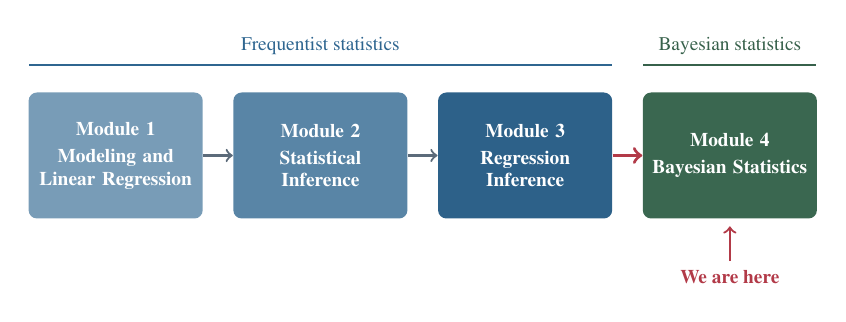
\begin{tikzpicture}[
    mod/.style={rectangle, rounded corners=3pt, minimum height=1.6cm, text width=2.0cm,
                align=center, font=\scriptsize\bfseries, text=white, inner sep=3pt}
  ]
  \node[mod, fill=ccBlue!65]        (m1) at (0,0)   {Module 1\\[2pt] Modeling and Linear Regression};
  \node[mod, fill=ccBlue!80]        (m2) at (2.6,0) {Module 2\\[2pt] Statistical Inference};
  \node[mod, fill=ccBlue!95!black]  (m3) at (5.2,0) {Module 3\\[2pt] Regression Inference};
  \node[mod, fill=ccGreen!75!black] (m4) at (7.8,0) {Module 4\\[2pt] Bayesian Statistics};

  \draw[->, thick, ccGray]   (m1) -- (m2);
  \draw[->, thick, ccGray]   (m2) -- (m3);
  \draw[->, very thick, ccRed] (m3) -- (m4);

  \draw[ccBlue, line width=1pt] (-1.1,1.15) -- (6.3,1.15)
    node[midway, above, font=\scriptsize, text=ccBlue] {Frequentist statistics};
  \draw[ccGreen!70!black, line width=1pt] (6.7,1.15) -- (8.9,1.15)
    node[midway, above, font=\scriptsize, text=ccGreen!70!black] {Bayesian statistics};

  \node[font=\scriptsize\bfseries, text=ccRed] (here) at (7.8,-1.55) {We are here};
  \draw[->, thick, ccRed] (here) -- (7.8,-0.9);
\end{tikzpicture}
\end{center}

\end{frame}

%%%%%%%%%%%%%%%%%%%%%%%%%%%%%%%%%%%%%%%%%%%%%%%%%%%%%%%%%%%%%%%%%%%%%%%%
\begin{frame}
\frametitle{How do you decide if you like a new restaurant?}

Imagine a new ramen restaurant just opened on Comm Ave.

\pause
\medskip

\dq{How do you decide whether it's any good?}

\pause

\begin{itemize}
\item Before you know anything: maybe you look at the Yelp rating: \textbf{2 reviews, 4.5 stars}
\pause
\item Then a friend eats there and says it was \textbf{just okay}
\pause
\item Then you eat there yourself and \textbf{like it a lot}
\pause
\item But when you go back with friends, it's \textbf{mediocre}
\end{itemize}

\pause
\medskip

Your opinion \emph{evolves} as you gather new information. You never started from scratch: each time you \textbf{updated} what you already believed.

\end{frame}

%%%%%%%%%%%%%%%%%%%%%%%%%%%%%%%%%%%%%%%%%%%%%%%%%%%%%%%%%%%%%%%%%%%%%%%%
\begin{frame}
\frametitle{Two meanings of ``probability''}

\dq{What do you mean when you say a coin lands heads with probability $1/2$?}

\pause

\textbf{Frequentist:} ``flip it over and over, half the flips land heads.'' Probability is the \hl{long-run frequency} of a repeatable event.

\pause
\medskip

\textbf{Bayesian:} ``flip it once, heads and tails are equally likely.'' Probability is a \hl{measure of plausibility}.

\pause
\medskip

Only the second can say ``70\% chance of rain tomorrow'': tomorrow does not repeat.

\end{frame}

%%%%%%%%%%%%%%%%%%%%%%%%%%%%%%%%%%%%%%%%%%%%%%%%%%%%%%%%%%%%%%%%%%%%%%%%
\begin{frame}
\frametitle{Bayesian knowledge building}

Take probability to mean plausibility, and the restaurant story becomes a method:

\medskip

\begin{center}
{\small
prior $\xrightarrow{\text{observe data}}$ posterior $\xrightarrow{\text{observe more data}}$ updated posterior $\longrightarrow \cdots$}
\end{center}

\pause
\medskip

\keyidea{Yesterday's posterior is today's prior. You never start over: each new piece of evidence updates what you already believed, and with enough data the early prior stops mattering.}

\pause
\medskip

\textbf{The restaurant:} the Yelp rating was your prior. Your friend's report, your own first meal, and the second visit were three rounds of data.

\end{frame}

%%%%%%%%%%%%%%%%%%%%%%%%%%%%%%%%%%%%%%%%%%%%%%%%%%%%%%%%%%%%%%%%%%%%%%%%
\section{Probability review}

%%%%%%%%%%%%%%%%%%%%%%%%%%%%%%%%%%%%%%%%%%%%%%%%%%%%%%%%%%%%%%%%%%%%%%%%
\begin{frame}
\frametitle{Events and probabilities}

A \hl{random experiment} is any process with an uncertain outcome. An \hl{event} is a possible outcome, or a set of outcomes.

\pause
\medskip

\begin{itemize}
\item \textbf{Flip a coin:} ``heads'', with $P(\text{heads}) = 0.5$.
\item \textbf{Screen a patient:} ``the test is positive'', with $P(\text{positive}) = 0.05$.
\item \textbf{Treat 6 patients:} ``exactly 2 respond'', with $P(2 \text{ respond}) = 0.32$.
\item \textbf{Detect a signal:} ``two neutron stars merged'', with $P(\text{BNS}) = 0.15$.
\end{itemize}

\pause
\medskip

The last three run through the whole lecture.

\end{frame}

%%%%%%%%%%%%%%%%%%%%%%%%%%%%%%%%%%%%%%%%%%%%%%%%%%%%%%%%%%%%%%%%%%%%%%%%
\begin{frame}
\frametitle{Rules of probability}

Write $P(A)$ for the probability that event $A$ occurs, and $A^c$ for ``$A$ does not occur''.

\pause
\medskip

\begin{itemize}
\item $0 \le P(A) \le 1$. \quad The test is positive with probability $0.05$, never $1.4$.
\pause
\item $P(A^c) = 1 - P(A)$. \quad So the test is negative with probability $0.95$.
\pause
\item $P(A \text{ or } B) = P(A) + P(B)$ when $A$ and $B$ are mutually exclusive. \quad A signal cannot be both BBH and BNS, so $P(\text{BBH or BNS}) = 0.65$.
\end{itemize}

\end{frame}

%%%%%%%%%%%%%%%%%%%%%%%%%%%%%%%%%%%%%%%%%%%%%%%%%%%%%%%%%%%%%%%%%%%%%%%%
\begin{frame}
\frametitle{Conditional probability}

The \hl{conditional probability} of $A$ given $B$ is the probability that $A$ occurs, given that we \textit{know} $B$ has occurred:
\[
P(A \mid B) = \frac{P(A \text{ and } B)}{P(B)}
\]
\pause
\medskip
\textbf{Roll a fair die.} $P(\text{six}) = 1/6$, but $P(\text{six} \mid \text{the roll is even}) = 1/3$.

\pause
\medskip
Equivalently, via the \textbf{multiplication rule}:
\[
P(A \text{ and } B) = P(A \mid B) \cdot P(B)
\]
\pause
\textbf{Independence:} $A$ and $B$ are independent if $P(A \mid B) = P(A)$, so knowing $B$ happened does not change the probability of $A$. Two rolls of the die are independent.

\end{frame}

%%%%%%%%%%%%%%%%%%%%%%%%%%%%%%%%%%%%%%%%%%%%%%%%%%%%%%%%%%%%%%%%%%%%%%%%
\begin{frame}
\frametitle{Law of total probability}

If events $B_1, B_2, \ldots, B_k$ are mutually exclusive and exhaustive (they cover all possibilities), then for any event $A$:
\[
P(A) = \sum_{i=1}^{k} P(A \mid B_i)\, P(B_i)
\]
\pause
\medskip
\textbf{Two groups.} Split the world into $B$ and its complement $B^c$:
\[
P(A) = P(A \mid B)\,P(B) + P(A \mid B^c)\,P(B^c)
\]
\pause
\medskip
This is useful when $P(A)$ is out of reach directly but is easy to write down scenario by scenario. On the next slides $A$ is ``the test came back positive'' and $B$ is ``the patient has the disease''.

\end{frame}

%%%%%%%%%%%%%%%%%%%%%%%%%%%%%%%%%%%%%%%%%%%%%%%%%%%%%%%%%%%%%%%%%%%%%%%%
\begin{frame}
\frametitle{Bayes' rule}

\textbf{Bayes' rule} lets us \textit{reverse} a conditional probability: we know $P(B \mid A)$, but what we want is $P(A \mid B)$.

\pause

\formula{Bayes' Rule}{\[P(A \mid B) = \frac{P(B \mid A) \, P(A)}{P(B)}\] and, when $P(B)$ is not directly available, expand the denominator with the law of total probability: \vspace{-0.4em}\[P(A \mid B) = \frac{P(B \mid A) \, P(A)}{P(B \mid A)\,P(A) + P(B \mid A^c)\,P(A^c)}.\]\vspace{-1.4em}}

\pause
\medskip

The two lines are the same rule. The second just writes the denominator out in full.

\end{frame}

%%%%%%%%%%%%%%%%%%%%%%%%%%%%%%%%%%%%%%%%%%%%%%%%%%%%%%%%%%%%%%%%%%%%%%%%
\section{Bayes' rule for events}

%%%%%%%%%%%%%%%%%%%%%%%%%%%%%%%%%%%%%%%%%%%%%%%%%%%%%%%%%%%%%%%%%%%%%%%%
\begin{frame}
\frametitle{Example: disease screening}

A rapid test for a rare disease. Write $D$ for having the disease and $+$ for a positive test.
\begin{itemize}
\item \textbf{Prevalence:} 1 in 1{,}000 have the disease, so the prior is $P(D) = 0.001$
\item \textbf{Sensitivity:} $P(+ \mid D) = 0.99$
\item \textbf{Specificity:} $P(\text{negative} \mid D^c) = 0.95$, so $P(+ \mid D^c) = 0.05$
\end{itemize}

\pause

\dq{You test positive. What is the chance you have the disease?}

\pause

\vspace{-0.3em}
{\footnotesize
\begin{align*}
P(D \mid +)
&= \frac{P(+ \mid D)\,P(D)}{P(+ \mid D)\,P(D) + P(+ \mid D^c)\,P(D^c)} \\[-0.2em]
&= \frac{0.99 \times 0.001}{0.99 \times 0.001 + 0.05 \times 0.999}
= \frac{0.00099}{0.05094} \approx \hl{0.019}
\end{align*}}

\end{frame}

%%%%%%%%%%%%%%%%%%%%%%%%%%%%%%%%%%%%%%%%%%%%%%%%%%%%%%%%%%%%%%%%%%%%%%%%
\begin{frame}
\frametitle{Why is the posterior so low?}
\examplehead{Disease screening}

Count out 1{,}000 people:
\begin{itemize}
\item about \textbf{1} has the disease, and tests positive $0.99$ of the time
\item about \textbf{999} are healthy, and $999 \times 0.05 \approx \textbf{50}$ of them test positive anyway
\end{itemize}
That is $0.99 + 49.95 = 50.94$ positives in all, of which only $0.99$ are real, so $0.99/50.94 \approx \hl{0.019}$.

\pause

\caution{A test being ``95\% accurate'' means little on its own. When the condition is rare, the false positives drawn from the huge healthy group outnumber the true positives from the tiny sick group.}

\end{frame}

%%%%%%%%%%%%%%%%%%%%%%%%%%%%%%%%%%%%%%%%%%%%%%%%%%%%%%%%%%%%%%%%%%%%%%%%
\begin{frame}
\frametitle{The prior does the work}
\examplehead{Disease screening}

\begin{center}
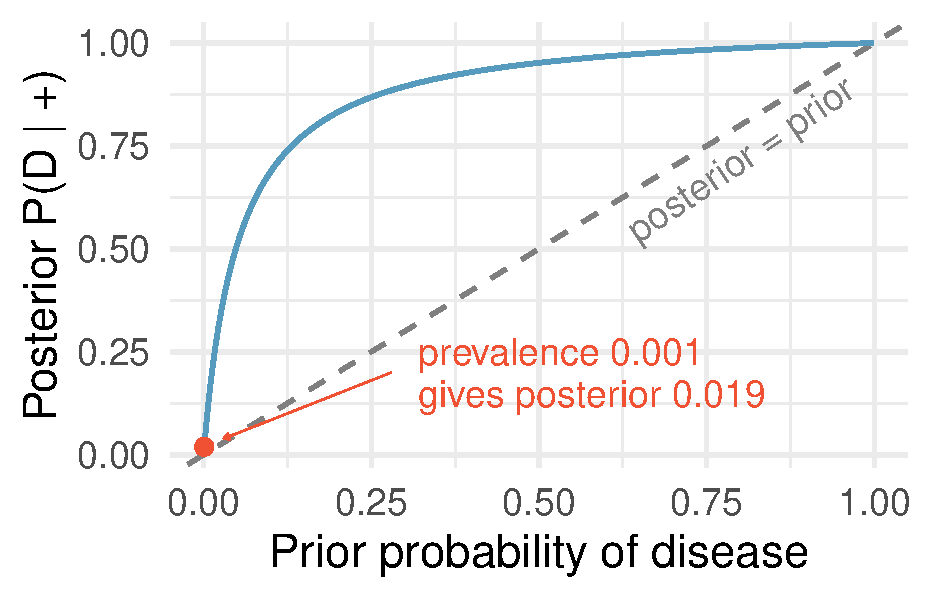
\includegraphics[width=0.68\textwidth]{posterior_vs_prior.pdf}
\end{center}

\vspace{-0.2em}
Every possible prior, same test. The posterior passes $0.5$ only once the prior passes about $0.05$.

\end{frame}

%%%%%%%%%%%%%%%%%%%%%%%%%%%%%%%%%%%%%%%%%%%%%%%%%%%%%%%%%%%%%%%%%%%%%%%%
\section{Conditional distributions and priors}

%%%%%%%%%%%%%%%%%%%%%%%%%%%%%%%%%%%%%%%%%%%%%%%%%%%%%%%%%%%%%%%%%%%%%%%%
\begin{frame}
\frametitle{From events to numbers}

Every unknown up to now has been an \hl{event}: the patient has the disease, or does not. Bayes' rule gives one probability for it.

\pause
\medskip

But most things we want to learn are \hl{numbers}: a response rate, a slope, a mean. There is no ``it happened or it didn't'' to pin a probability on.

\pause

\keyidea{So put the prior on the \emph{number} itself, spreading probability across the values it could take. The prior stops being one number and becomes a whole distribution, and so does the posterior. Everything else (multiply by the likelihood, then normalize) is unchanged.}

\end{frame}

%%%%%%%%%%%%%%%%%%%%%%%%%%%%%%%%%%%%%%%%%%%%%%%%%%%%%%%%%%%%%%%%%%%%%%%%
\begin{frame}
\frametitle{Example: a Phase 1 drug trial}

A biotech company is running a small Phase 1 trial of a new cancer drug on $n = 6$ patients.\footnote{\scriptsize The FDA has \underline{\href{https://www.fda.gov/regulatory-information/search-fda-guidance-documents/use-bayesian-methodology-clinical-trials-drug-and-biological-products}{draft guidance}} on Bayesian methods in clinical trials.} \textbf{Data:} $x = 2$ of the 6 respond. Let
\[
p = \text{probability that a patient responds to the drug.}
\]
\pause
\dq{What should we now believe about $p$?}

\pause
Two ingredients:
\begin{enumerate}
\item A \hl{data model} (likelihood): how likely is the data under each value of $p$?
\item A \hl{prior}: what did we believe about $p$ \textbf{before} the trial?
\end{enumerate}

\end{frame}

%%%%%%%%%%%%%%%%%%%%%%%%%%%%%%%%%%%%%%%%%%%%%%%%%%%%%%%%%%%%%%%%%%%%%%%%
\begin{frame}
\frametitle{Random variables}

A \hl{random variable} $X$ is a numerical quantity whose value depends on the outcome of a random process.

\pause
\medskip

A \textbf{discrete} random variable takes values in a countable set (e.g.\ $\{0, 1, \dots, n\}$), and is described by a \hl{probability mass function} (PMF), which says how much probability sits on each possible value:
\[
P(X = x) = f(x), \qquad \sum_x f(x) = 1.
\]
\pause
\textbf{The Bayesian move:} treat the unknown parameter $p$ \emph{itself} as a random variable, with its own distribution $f(p)$. In the frequentist framework $p$ is a fixed constant and only the data is random.

\end{frame}

%%%%%%%%%%%%%%%%%%%%%%%%%%%%%%%%%%%%%%%%%%%%%%%%%%%%%%%%%%%%%%%%%%%%%%%%
\begin{frame}
\frametitle{Bayes' rule for random variables}

The same rule applies with \emph{random variables} in place of events. If $p$ is the unknown parameter and $x$ the data:
\[
\underbrace{f(p \mid x)}_{\text{posterior}} \;=\; \frac{\overbrace{f(x \mid p)}^{\text{likelihood}}\;\overbrace{f(p)}^{\text{prior}}}{\underbrace{f(x)}_{\text{evidence}}}
\]
\pause

\formula{Notation}{$f(\cdot)$ denotes a probability mass function. $f(p)$ is the \hl{prior}: what we believe before the trial. $f(x \mid p)$ is the \hl{likelihood}: how probable $x$ is when the response rate is $p$. Read as a function of $p$ we write it $L(p ; x)$. $f(p \mid x)$ is the \hl{posterior}: what we believe having seen $x$.}

\end{frame}

%%%%%%%%%%%%%%%%%%%%%%%%%%%%%%%%%%%%%%%%%%%%%%%%%%%%%%%%%%%%%%%%%%%%%%%%
\begin{frame}
\frametitle{The evidence is just a normalizing constant}

The denominator $f(x)$, the \textbf{marginal likelihood}, does not depend on $p$. It is the same number for every candidate value of $p$, so all it does is rescale the numerator to make the posterior sum to one:
\[
f(x) \;=\; \sum_p f(x \mid p)\, f(p).
\]
That is the law of total probability, now summing over candidate values of $p$ rather than over events.

\pause

So we usually drop it and write
\[
f(p \mid x) \;\propto\; f(x \mid p)\, f(p) \;=\; L(p ; x)\, f(p).
\]
\pause
\begin{center}
\textbf{Posterior $\propto$ likelihood $\times$ prior.}
\end{center}

\end{frame}

%%%%%%%%%%%%%%%%%%%%%%%%%%%%%%%%%%%%%%%%%%%%%%%%%%%%%%%%%%%%%%%%%%%%%%%%
\begin{frame}
\frametitle{The binomial likelihood}
\examplehead{Phase 1 drug trial}

If $n$ patients independently respond with probability $p$, then $X \mid p \sim \text{Binomial}(n, p)$:
\[
P(X = x \mid p) = \binom{n}{x} p^x (1 - p)^{n - x}
\]
\pause
Evaluate the \hl{likelihood} at five candidate values of $p$ ($n = 6$, $x = 2$):
\[
{\scriptsize
\begin{array}{c|c|c}
p & \binom{6}{2}p^2(1-p)^4 & L(p ; x = 2) \\
\hline
0.1 & 15\,(0.1)^2(0.9)^4 & 0.098 \\
0.3 & 15\,(0.3)^2(0.7)^4 & 0.324 \\
0.5 & 15\,(0.5)^2(0.5)^4 & 0.234 \\
0.7 & 15\,(0.7)^2(0.3)^4 & 0.060 \\
0.9 & 15\,(0.9)^2(0.1)^4 & 0.001 \\
\end{array}}
\]
\vspace{-0.6em}
The likelihood peaks at $p = 0.3$, near the observed $2/6$.

\end{frame}

%%%%%%%%%%%%%%%%%%%%%%%%%%%%%%%%%%%%%%%%%%%%%%%%%%%%%%%%%%%%%%%%%%%%%%%%
\begin{frame}
\frametitle{Bringing in the prior}
\examplehead{Phase 1 drug trial}

The likelihood ranks values of $p$ by the \emph{data} alone, ignoring what we already know about drugs in this class.

\pause
\medskip
\textbf{Prior knowledge.} Most early-stage oncology drugs respond poorly, moderate response is uncommon, and strong response is rare. Encode that over the same grid:

\begin{center}
\renewcommand{\arraystretch}{1.1}
\begin{tabular}{c|ccccc}
\toprule
$p$     & 0.1  & 0.3  & 0.5  & 0.7  & 0.9  \\
\midrule
$f(p)$  & 0.45 & 0.30 & 0.15 & 0.07 & 0.03 \\
\bottomrule
\end{tabular}
\end{center}

\pause
This is a \hl{probability distribution on a parameter}, the move that makes an analysis Bayesian.

\end{frame}

%%%%%%%%%%%%%%%%%%%%%%%%%%%%%%%%%%%%%%%%%%%%%%%%%%%%%%%%%%%%%%%%%%%%%%%%
\begin{frame}
\frametitle{Computing the posterior}
\examplehead{Phase 1 drug trial}

\vspace{0.35em}
\begin{center}
\renewcommand{\arraystretch}{1.15}
\begin{tabular}{c c c c c}
\toprule
$p$ & Prior $f(p)$ & Likelihood $L(p ; x)$ & Product & Posterior $f(p\mid x)$ \\
\midrule
0.1 & 0.45 & 0.098 & 0.044 & 0.245 \\
0.3 & 0.30 & 0.324 & 0.097 & \textbf{0.538} \\
0.5 & 0.15 & 0.234 & 0.035 & 0.194 \\
0.7 & 0.07 & 0.060 & 0.004 & 0.023 \\
0.9 & 0.03 & 0.001 & 0.000 & $\approx 0$ \\
\midrule
\multicolumn{3}{r}{Total:} & 0.181 & 1.000 \\
\bottomrule
\end{tabular}
\end{center}
\pause
\begin{center}
\small Prior mean $E(p) = 0.29$ \hspace{1.5em} $\longrightarrow$ \hspace{1.5em} Posterior mean $E(p \mid x) = 0.30$
\end{center}
\end{frame}

%%%%%%%%%%%%%%%%%%%%%%%%%%%%%%%%%%%%%%%%%%%%%%%%%%%%%%%%%%%%%%%%%%%%%%%%
\begin{frame}
\frametitle{What if 5 of 6 patients responded?}
\examplehead{Phase 1 drug trial}

\hl{Likelihood:} $L(p ; x=5) = \binom{6}{5} p^5 (1-p)$

\pause

\vspace{-0.2em}
\begin{center}
{\small
\renewcommand{\arraystretch}{1.1}
\begin{tabular}{c c c c c}
\toprule
$p$ & Prior $f(p)$ & Likelihood $L(p ; x)$ & Product & Posterior $f(p\mid x)$ \\
\midrule
0.1 & 0.45 & 0.0001 & 0.0000 & $\approx 0$ \\
0.3 & 0.30 & 0.0102 & 0.0031 & 0.063 \\
0.5 & 0.15 & 0.0938 & 0.0141 & 0.287 \\
0.7 & 0.07 & 0.3025 & 0.0212 & \textbf{0.433} \\
0.9 & 0.03 & 0.3543 & 0.0106 & 0.217 \\
\midrule
\multicolumn{3}{r}{Total:} & 0.0490 & 1.000 \\
\bottomrule
\end{tabular}}
\end{center}
\pause
\begin{center}
\small Prior mean $E(p) = 0.29$ \hspace{1.5em} $\longrightarrow$ \hspace{1.5em} Posterior mean $E(p \mid x) = 0.66$
\end{center}

\end{frame}

%%%%%%%%%%%%%%%%%%%%%%%%%%%%%%%%%%%%%%%%%%%%%%%%%%%%%%%%%%%%%%%%%%%%%%%%
\begin{frame}
\frametitle{Same prior, different data}
\examplehead{Phase 1 drug trial}

\begin{center}
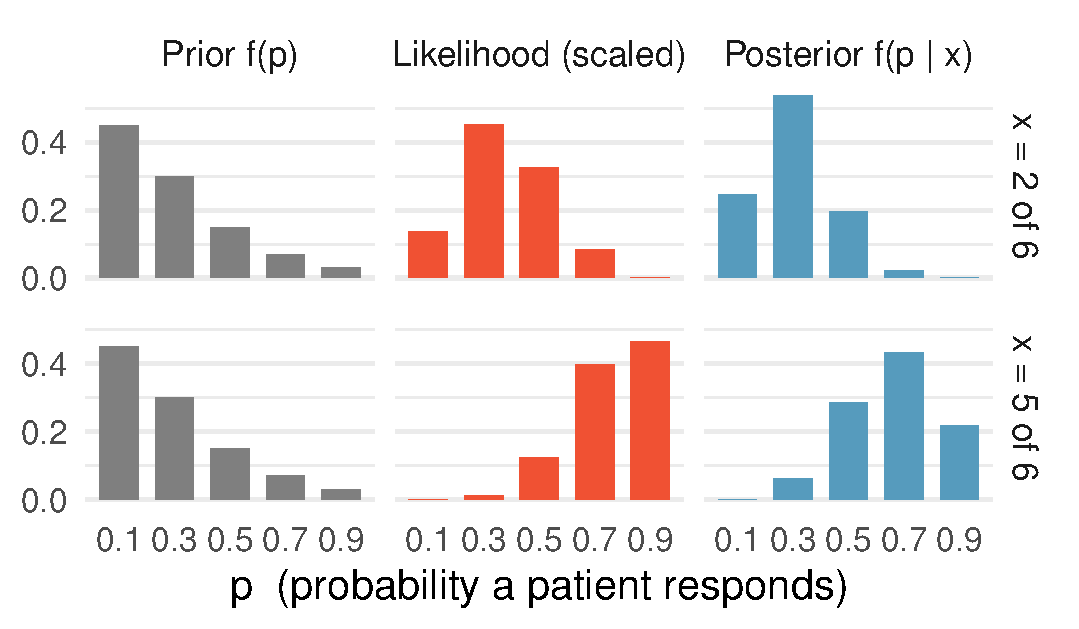
\includegraphics[width=0.84\textwidth]{drug_trial_update.pdf}
\end{center}

\vspace{-0.5em}
Identical prior in both rows. The data alone moves the posterior.

\end{frame}

%%%%%%%%%%%%%%%%%%%%%%%%%%%%%%%%%%%%%%%%%%%%%%%%%%%%%%%%%%%%%%%%%%%%%%%%
\section{Sequentiality and updating}

%%%%%%%%%%%%%%%%%%%%%%%%%%%%%%%%%%%%%%%%%%%%%%%%%%%%%%%%%%%%%%%%%%%%%%%%
\begin{frame}
\frametitle{Updating with more data}
\examplehead{Disease screening}

One positive test put the chance of disease at $0.019$.

\pause
\dq{What if you take the test a second time and it's positive again?}

\pause

\textbf{Yesterday's posterior is today's prior.} That $0.019$ is what we believe now, so it becomes the prior for the second test:

\vspace{-0.3em}
\[
P(D \mid +_2) = \frac{0.99 \times 0.019}{0.99 \times 0.019 + 0.05 \times 0.981} = \frac{0.01881}{0.06786} \approx \hl{0.28}
\]
\pause
After a third \textbf{independent} positive test: $P(D \mid +_3) \approx \hl{0.88}$.

\pause

It takes three positive tests for the evidence to outweigh the low prior.

\end{frame}

%%%%%%%%%%%%%%%%%%%%%%%%%%%%%%%%%%%%%%%%%%%%%%%%%%%%%%%%%%%%%%%%%%%%%%%%
\begin{frame}
\frametitle{Example: classifying a gravitational-wave signal}

In 2017 \hl{LIGO} detected a gravitational wave, a ripple in spacetime from a violent astrophysical event. \dq{What produced it?}

\pause

\textbf{Four possible sources}, with priors based on expected rates:

\renewcommand{\arraystretch}{1.15}
\begin{tabular}{l l l}
BBH & Binary black hole merger & $P(\text{BBH}) = 0.50$ \\
BNS & Binary neutron star merger & $P(\text{BNS}) = 0.15$ \\
NSBH & Neutron star--black hole & $P(\text{NSBH}) = 0.10$ \\
Noise & Detector glitch & $P(\text{Noise}) = 0.25$
\end{tabular}

\pause
\medskip

Those four numbers are a \hl{prior distribution}, as in the trial but over four hypotheses.

\end{frame}

%%%%%%%%%%%%%%%%%%%%%%%%%%%%%%%%%%%%%%%%%%%%%%%%%%%%%%%%%%%%%%%%%%%%%%%%
\begin{frame}
\frametitle{First observation: signal duration}
\examplehead{Gravitational-wave signal}

The detected signal lasts more than 1 second (``long'').

\pause
\medskip

How likely is a long signal under each source type?
\begin{itemize}
\item $P(\text{long} \mid \text{BBH}) = 0.20$ \quad (BBH signals are typically short)
\item $P(\text{long} \mid \text{BNS}) = 0.90$ \quad (neutron stars spiral slowly)
\item $P(\text{long} \mid \text{NSBH}) = 0.50$
\item $P(\text{long} \mid \text{Noise}) = 0.35$
\end{itemize}

\pause
\medskip

Apply Bayes' rule to each hypothesis $H_i$, one of the four sources:
\[
P(H_i \mid \text{long})
=  \frac{P(\text{long} \mid H_i) \cdot P(H_i)}{P(\text{long})}
= \frac{P(\text{long} \mid H_i) \cdot P(H_i)}{\sum_{j} P(\text{long} \mid H_j) \cdot P(H_j)}
\]

\end{frame}

%%%%%%%%%%%%%%%%%%%%%%%%%%%%%%%%%%%%%%%%%%%%%%%%%%%%%%%%%%%%%%%%%%%%%%%%
\begin{frame}
\frametitle{Posterior after signal duration}
\examplehead{Gravitational-wave signal}

\begin{center}
\renewcommand{\arraystretch}{1.15}
\begin{tabular}{l c c c c}
\toprule
Source & Prior & Likelihood & Product & Posterior \\
\midrule
BBH  & 0.50 & 0.20 & 0.100 & 0.268 \\
BNS  & 0.15 & 0.90 & 0.135 & \textbf{0.362} \\
NSBH & 0.10 & 0.50 & 0.050 & 0.134 \\
Noise & 0.25 & 0.35 & 0.088 & 0.235 \\
\midrule
& & Total: &  0.373 & 1.000 \\
\bottomrule
\end{tabular}
\end{center}

\pause
\medskip

BNS rose from 15\% to 36\% and BBH dropped from 50\% to 27\%. No hypothesis is above 40\%, so the signal is not yet classified.

\end{frame}

%%%%%%%%%%%%%%%%%%%%%%%%%%%%%%%%%%%%%%%%%%%%%%%%%%%%%%%%%%%%%%%%%%%%%%%%
\begin{frame}
\frametitle{Second observation: electromagnetic counterpart}
\examplehead{Gravitational-wave signal}

Astronomers point telescopes at the source location and detect a \hl{kilonova}: a burst of light produced when neutron star matter is ejected during a merger.

\pause
\medskip

How likely is an EM counterpart under each source type?
\begin{itemize}
\item $P(\text{EM} \mid \text{BBH}) = 0.01$ \quad (black holes produce no light)
\item $P(\text{EM} \mid \text{BNS}) = 0.80$ \quad (neutron star mergers produce kilonovae)
\item $P(\text{EM} \mid \text{NSBH}) = 0.20$ \quad (possible, but less likely than BNS)
\item $P(\text{EM} \mid \text{Noise}) = 0.02$ \quad (coincidental)
\end{itemize}

\pause

The posterior after the duration becomes the prior for this update.

\end{frame}

%%%%%%%%%%%%%%%%%%%%%%%%%%%%%%%%%%%%%%%%%%%%%%%%%%%%%%%%%%%%%%%%%%%%%%%%
\begin{frame}
\frametitle{Posterior after the EM counterpart}
\examplehead{Gravitational-wave signal}

\vspace{0.35em}
\renewcommand{\arraystretch}{1.15}
\begin{tabular}{l c c c c}
\toprule
Source & Prior (from before) & Likelihood & Product & Posterior \\
\midrule
BBH  & 0.268 & 0.01 & 0.003 & 0.008 \\
BNS  & 0.362 & 0.80 & 0.290 & \textbf{0.894} \\
NSBH & 0.134 & 0.20 & 0.027 & 0.083 \\
Noise & 0.235 & 0.02 & 0.005 & 0.014 \\
\midrule
& & Total:  & 0.324 & 1.000 \\
\bottomrule
\end{tabular}

\pause
\medskip

A binary neutron star merger now has posterior probability 89\%, mirroring the real analysis of \hl{GW170817}.

\end{frame}

%%%%%%%%%%%%%%%%%%%%%%%%%%%%%%%%%%%%%%%%%%%%%%%%%%%%%%%%%%%%%%%%%%%%%%%%
\begin{frame}
\frametitle{Order doesn't matter}
\examplehead{Gravitational-wave signal}

\dq{What if the telescopes had reported before the duration was measured?}

\pause

\begin{center}
{\small
\renewcommand{\arraystretch}{1.05}
\begin{tabular}{l c c}
\toprule
Source & Duration, then EM & EM, then duration \\
\midrule
BBH  & 0.008 & 0.008 \\
BNS  & \textbf{0.894} & \textbf{0.894} \\
NSBH & 0.083 & 0.083 \\
Noise & 0.014 & 0.014 \\
\bottomrule
\end{tabular}}
\end{center}

\pause

\textbf{Why?} Each update multiplies by a likelihood, and the product is the same either way.

\end{frame}

%%%%%%%%%%%%%%%%%%%%%%%%%%%%%%%%%%%%%%%%%%%%%%%%%%%%%%%%%%%%%%%%%%%%%%%%
\begin{frame}
\frametitle{Order doesn't matter}
\examplehead{Gravitational-wave signal}

\begin{center}
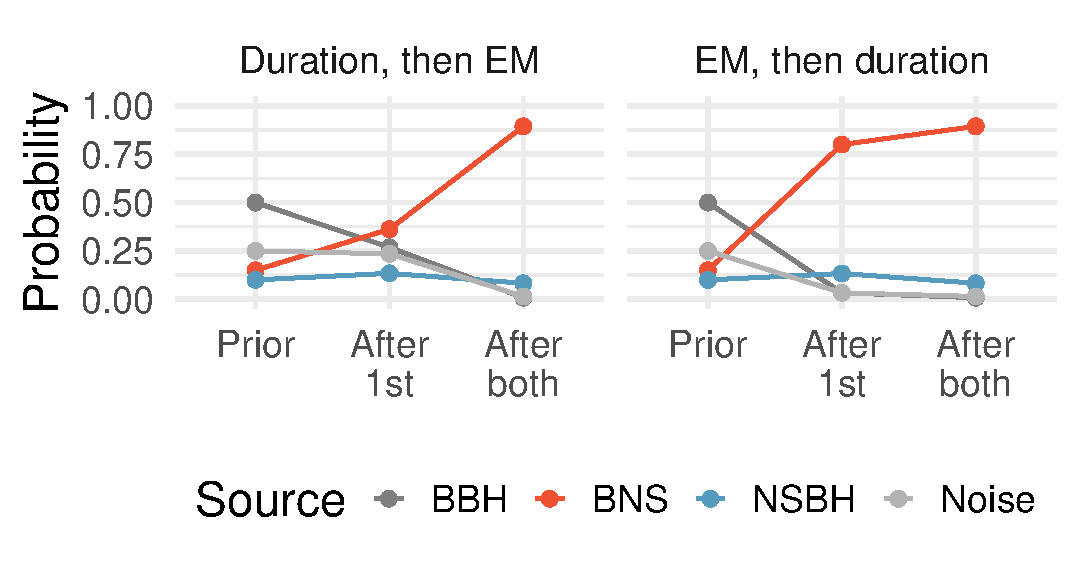
\includegraphics[width=0.74\textwidth]{order_invariance.pdf}
\end{center}

\vspace{-0.6em}
\keyidea{After one observation the two routes disagree completely. The destination is the same.}

\end{frame}

%%%%%%%%%%%%%%%%%%%%%%%%%%%%%%%%%%%%%%%%%%%%%%%%%%%%%%%%%%%%%%%%%%%%%%%%
\section{Bayesian vs.\ frequentist}

%%%%%%%%%%%%%%%%%%%%%%%%%%%%%%%%%%%%%%%%%%%%%%%%%%%%%%%%%%%%%%%%%%%%%%%%
\begin{frame}
\frametitle{Hypothesis testing: the frequentist question}
\examplehead{Disease screening}

One positive test, with the original numbers: $P(D) = 0.001$, sensitivity $0.99$, specificity $0.95$. Take $H_0$: the patient is healthy.

\medskip
\textbf{Frequentist:} \emph{how surprising is this data if $H_0$ is true?}
\begin{itemize}
\item $p\text{-value} = P(+ \mid H_0) = 0.05$
\pause
\item \hl{$s$-value} $= -\log_2(p) \approx 4.3$ \hl{bits of evidence against $H_0$}
\item About as surprising as getting 4 heads in a row
\end{itemize}

\pause
\medskip

On its own terms that is a real signal: a healthy patient tests positive only 1 time in 20.

\end{frame}

%%%%%%%%%%%%%%%%%%%%%%%%%%%%%%%%%%%%%%%%%%%%%%%%%%%%%%%%%%%%%%%%%%%%%%%%
\begin{frame}
\frametitle{Hypothesis testing: the Bayesian question}
\examplehead{Disease screening}

\textbf{Bayesian:} \emph{how likely is $H_0$ given this data?}
\begin{itemize}
\item $P(H_0 \mid +) = 1 - P(D \mid +) \approx \hl{0.98}$
\item The patient is almost certainly healthy, because the prior was so low
\end{itemize}

\pause
We can form a \hl{Bayesian $p$-value} and \hl{$s$-value} from the posterior:
\[
p_{\text{Bayes}} = P(H_0 \mid \text{data}), \qquad s_{\text{Bayes}} = -\log_2 p_{\text{Bayes}}.
\]
So $s_{\text{Bayes}} \approx 0.03$ bits: essentially \emph{no} evidence against $H_0$.

\pause
\hl{4.3 bits against, or 0.03 bits against?} The two answer \emph{different questions}.

\end{frame}

%%%%%%%%%%%%%%%%%%%%%%%%%%%%%%%%%%%%%%%%%%%%%%%%%%%%%%%%%%%%%%%%%%%%%%%%
\begin{frame}
\frametitle{Frequentist vs.\ Bayesian: key differences}

\renewcommand{\arraystretch}{1.3}
\begin{center}
{\small
\begin{tabular}{>{\raggedright\arraybackslash}p{2.1cm} >{\raggedright\arraybackslash}p{3.6cm} >{\raggedright\arraybackslash}p{3.6cm}}
\toprule
 & \textbf{Frequentist} & \textbf{Bayesian} \\
\midrule
\textbf{Probability} & Long-run frequency of a repeatable event & Degree of belief or plausibility \\
\textbf{Parameters} & Fixed but unknown constants & Random quantities with distributions \\
\textbf{Prior info} & Not formally used, held to be more ``objective'' & Encoded as a prior distribution \\
\textbf{Inference} & CIs, p-values, point estimates & Posterior distributions \\
\bottomrule
\end{tabular}}
\end{center}

\end{frame}

%%%%%%%%%%%%%%%%%%%%%%%%%%%%%%%%%%%%%%%%%%%%%%%%%%%%%%%%%%%%%%%%%%%%%%%%
\begin{frame}
\frametitle{So which should you use?}

With plenty of data the two usually agree, and the frequentist answer is cheaper to compute.

\pause
\medskip

Bayesian methods are worth the extra effort when:
\begin{itemize}
\item data is \hl{scarce} but you know something beforehand, as with 6 patients in a Phase 1 trial;
\pause
\item evidence \hl{arrives over time} and you must act as it does, as with the LIGO alert;
\pause
\item you need the probability of a \hl{hypothesis}, not the probability of the \hl{data}.
\end{itemize}

\pause
\medskip

When the prior is doing most of the work, say so. That is a feature, not something to hide.

\end{frame}

%%%%%%%%%%%%%%%%%%%%%%%%%%%%%%%%%%%%%%%%%%%%%%%%%%%%%%%%%%%%%%%%%%%%%%%%
\section{Wrap-up}

%%%%%%%%%%%%%%%%%%%%%%%%%%%%%%%%%%%%%%%%%%%%%%%%%%%%%%%%%%%%%%%%%%%%%%%%
\begin{frame}
\frametitle{Summary}

\begin{itemize}
\item The \hl{Bayesian approach} combines a prior with data to produce a posterior, the same way you update an opinion.
\pause
\item \hl{Bayes' rule} reverses a conditional probability, for events, for random variables, and for \hl{any number of hypotheses}:
\vspace{-0.3em}
\[
P(A \mid B) = \frac{P(B \mid A)\,P(A)}{P(B)}, \qquad f(p \mid x) \propto L(p ; x)\, f(p).
\]
\pause
\vspace{-0.5em}
\item Putting a \hl{prior distribution on a parameter} is the move that makes an analysis Bayesian.
\pause
\item We update \hl{sequentially}, and the final posterior doesn't depend on the order of the data.
\pause
\item With more data the \hl{posterior is increasingly driven by the data} rather than the prior.
\end{itemize}

\end{frame}

%%%%%%%%%%%%%%%%%%%%%%%%%%%%%%%%%%%%%%%%%%%%%%%%%%%%%%%%%%%%%%%%%%%%%%%%
\begin{frame}
\frametitle{Coming up next}

\begin{itemize}
\item \hl{Lecture 18 continues Module 4.} The parameter $p$ can be anything in $[0,1]$, not just the five values used today, so the prior becomes a \hl{continuous} curve: the \hl{Beta distribution}. Prior and posterior then share a shape, which makes it a \hl{conjugate model} (BR!\ Chs.\ 3 and 5).
\item \hl{Credible intervals} arrive with it. Read straight off the posterior, a 95\% credible interval is one the parameter falls in with probability $0.95$, which is what a confidence interval is usually misread as meaning. Lecture 20 covers them in full.
\end{itemize}

\end{frame}

%%%%%%%%%%%%%%%%%%%%%%%%%%%%%%%%%%%%%%%%%%%%%%%%%%%%%%%%%%%%%%%%%%%%%%%%
% Activity
%%%%%%%%%%%%%%%%%%%%%%%%%%%%%%%%%%%%%%%%%%%%%%%%%%%%%%%%%%%%%%%%%%%%%%%%

\begin{frame}
\frametitle{In-class activity}

You'll work in \textbf{pairs} (one analyst, one guide).

\medskip
\begin{itemize}
\item Pick up the worksheet.
\item Work through the problems together.
\item \hl{Don't use Gen AI except for debugging}
\item Your worksheet will be collected and graded.
\end{itemize}

\medskip
\textbf{Recommendations:}
\begin{itemize}
\item Read each question carefully before starting
\item Discuss your answers with your partner before writing them down.
\end{itemize}

\end{frame}

\end{document}
